\documentclass[tikz,border=6pt]{standalone}
\usepackage[utf8]{inputenc}
\usepackage[T1]{fontenc}
\usepackage{tikz}
\begin{document}
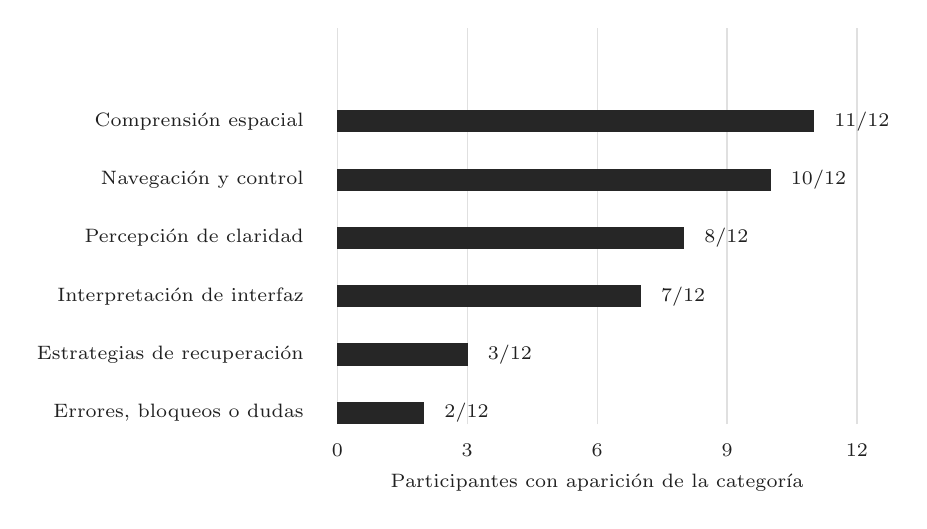
\begin{tikzpicture}[x=0.55cm,y=0.74cm,font=\sffamily]
  \definecolor{ink}{RGB}{32,32,32}
  \definecolor{soft}{RGB}{224,224,224}
  \definecolor{bar}{RGB}{38,38,38}

  \foreach \x in {0,3,6,9,12} {
    \draw[soft, line width=0.4pt] (\x,-0.2) -- (\x,6.6);
    \node[ink, font=\scriptsize] at (\x,-0.65) {\x};
  }
  \node[ink, font=\scriptsize] at (6,-1.2) {Participantes con aparición de la categoría};

  \foreach \label/\value/\row in {
    {Comprensión espacial}/11/5,
    {Navegación y control}/10/4,
    {Percepción de claridad}/8/3,
    {Interpretación de interfaz}/7/2,
    {Estrategias de recuperación}/3/1,
    {Errores, bloqueos o dudas}/2/0
  } {
    \node[anchor=east, ink, font=\scriptsize] at (-0.55,\row) {\label};
    \draw[fill=bar, draw=bar] (0,\row-0.18) rectangle (\value,\row+0.18);
    \node[anchor=west, ink, font=\scriptsize] at (\value+0.25,\row) {\value/12};
  }
\end{tikzpicture}
\end{document}
